\documentclass[12pt]{article}
\usepackage{amsmath} %a widely used math package
\usepackage{hyperref} %for hyperlinks
\usepackage{enumitem} %for (a) (b) (c) enumeration
\usepackage{fullpage} %sets the margins to 1 inch. Turn off for the more restrictive TeX default

%fonts:
\usepackage[]{newtx} %Times New Roman, in square brackets, try ebgaramond
%\usepackage{newpxtext,eulerpx} %Palatino + Euler
%\usepackage{kpfonts} %Johannes Kepler fonts
%\usepackage{kmath,kerkis} %Bookman Old Style

%\usepackage[default]{comicneue}
%\usepackage[T1]{fontenc}
%\usepackage[eulergreek,EULERGREEK]{sansmath}
%\sansmath

\usepackage[
backend=biber,
style=phys,
sorting=none,
]{biblatex}
\addbibresource{refs.bib}%path to bib file

\usepackage{xcolor}
\definecolor{burntorange}{RGB}{191,87,0}
\definecolor{bluebonnet}{RGB}{0,95,196}
\definecolor{charcoal}{RGB}{51,63,72}
\definecolor{solarized}{HTML}{FDF6E3}

\usepackage{lipsum}
\usepackage[symbol]{footmisc}
\usepackage{hyperref}
\hypersetup{
colorlinks=true,
%filecolor=bluebonnet,    
linkcolor=burntorange,
urlcolor=bluebonnet,
citecolor=bluebonnet
} 
\urlstyle{same}
\usepackage{graphicx}
\usepackage{tkz-euclide}
\usepackage{halloweenmath}

\usepackage{empheq}
\usepackage[most]{tcolorbox}
\newtcolorbox{feature}{
    enhanced,
    breakable,
    colback=solarized,
    colframe=burntorange,
    arc=0mm,
    boxrule=0.75pt, 
    drop fuzzy shadow southeast
}

\newtcbox{\eq}[1][]{%
	nobeforeafter, math upper, tcbox raise base,
	enhanced, colframe=burntorange,
	colback=solarized, boxrule=0.75pt, #1, drop fuzzy shadow southeast} %boxsep=-1mm

\renewcommand{\vec}[1]{\boldsymbol{\mathrm{#1}}}  
\newcommand\dyad[1]{\underline{\boldsymbol{\mathsf{#1}}}}
\newcommand{\nablav}{\boldsymbol{\nabla}}
\renewcommand{\Re}{\operatorname{Re}}  
\renewcommand{\Im}{\operatorname{Im}}  

\title{Sample \LaTeX\space document}
\author{Your Name \(\mathbat\)}
\date{\today} 

\begin{document}
\maketitle

\section{Introductory section} %you can use \subsection, etc. \section* removes the number
This is a sample document. The general solution of the Helmholtz equation in cylindrical coordinates \((r,\theta,z)\) is \cite[Eq.~(A--14)]{blackstock2000fundamentals}
%
\begin{align}\label{eq:eig}
\tilde{p}(r,\theta,z) &= p_0 [C_1J_\ell (k_rr) + C_2N_\ell(k_rr)] e^{i(\ell \theta + k_zz)}\,,\\
k &= \sqrt{k_r^2 + k_z^2}\,,
\end{align}
%
where \(p = \Im(\tilde{p}e^{-i\omega t})\) is the solution of the wave equation for angular frequency \(\omega\), \(p_0\) is the pressure amplitude, \(C_1\) and \(C_2\) are dimensionless constants, and \(J_\ell\) and \(N_\ell\) are the \(\ell\)th order Bessel and Neumann functions, respectively. The Pythagorean theorem is
%
\begin{empheq}[box=\eq]{align}\label{eq:pythag}
a^2 + b^2 = c^2\,.
\end{empheq}
%
Equation~\eqref{eq:pythag} is one of the most famous equations of mathematics. \lipsum[1-3]
%
\begin{figure}
\centering
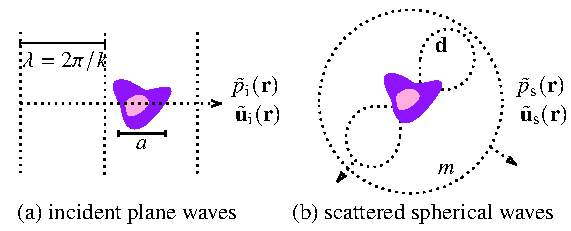
\includegraphics[width=0.63\linewidth]{figure}
\caption{Incident and scattered waves}\label{fig:Delta}
\end{figure}

\printbibliography
\end{document}
